
\chapter{Getting Started}

The Consolidated Model of Fire and Smoke Transport (CFAST) is documented by four publications, this user's guide, a technical reference guide~\cite{CFAST_Tech_Guide_7} a verification and validation guide \cite{CFAST_Valid_Guide_7}, and a configuration management guide~\cite{CFAST_Config_Guide_7}. The technical reference guide describes the underlying physical principles, provides a comparison with other models, and includes an evaluation of the model following the guidelines of ASTM~E1355~\cite{ASTM:E1355}. The model verification and validation guide documents verification and validation efforts for the model. The configuration management guide documents the processes used during the development and validation of the model. This user's guide describes how to use the model and the input editor CEdit.

\section{Installation}

The installation of CFAST is made up of thre programs. The main program, CFAST, is written in Fortran and can be run as a stand alone command line application that reads input data from a text file. It has been compiled and run on a number of different operating systems but the version in the distribution was compiled to run under Windows. The input editor, CEdit, that is distributed with CFAST is designed to run on a Windows platform. Also the version of the visualization software, Smokeview, is compiled to run on Windows. All of the files associated with CFAST can be obtained at: \url{http://cfast.nist.gov}

The CFAST distribution consists of a self-extracting set-up program for Windows-based personal computers. After downloading the set-up program, double-clicking on the file's icon walks you through a series of steps for installation of the program.  The most important part of the installation is the creation of a folder ({\ct C:$\backslash$Program Files$\backslash$CFAST} by default) in which the CFAST executable files and supplemental data files are installed.  Sample input files are found in the {\ct Examples} folder.

CFAST input files are best created and run using a Windows-based input editor called CEdit. Sample input files are provided with the program for new users who are encouraged to first run the sample calculations before attempting to create an input file. To run the model, browse to the location of the CFAST sample input file (default location is in a folder called {\ct Examples} in the installation folder) copy the file named {\ct Users\_Guide\_Example.in} to a location of your choice and then double click on the copied file. This should open the file in the CFAST input editor, CEdit, as shown in Fig.~\ref{primary_screen}.
\begin{figure}[h!]
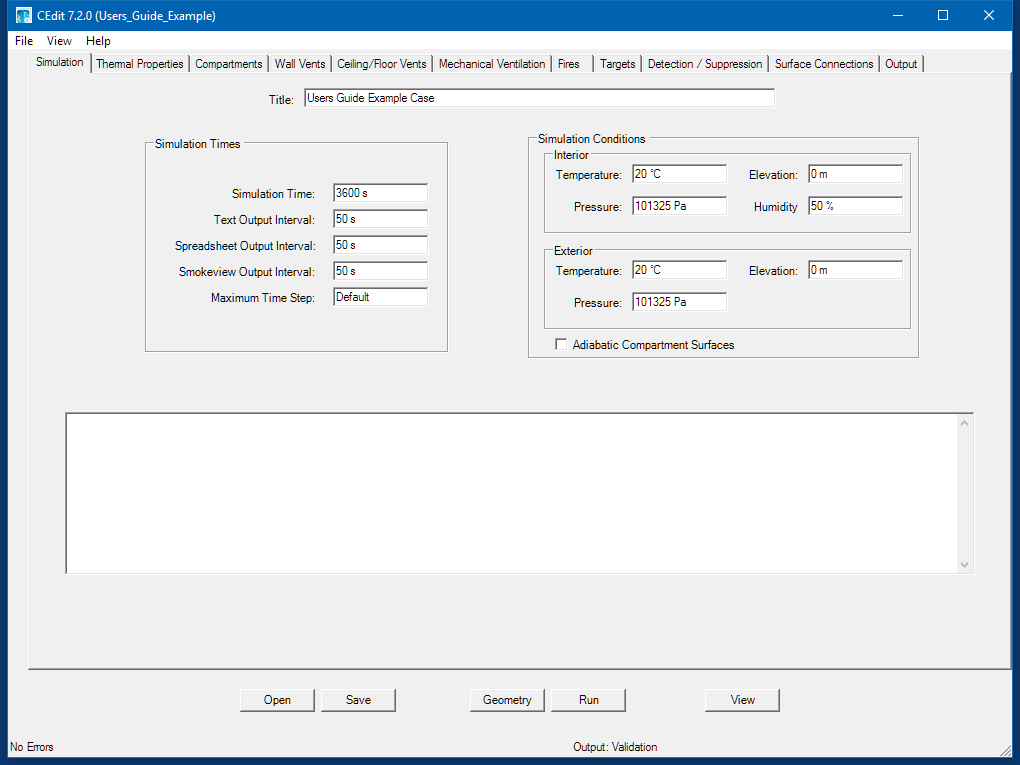
\includegraphics[width=6.5in]{FIGURES/Environment_Tab}
\caption[The Primary CFAST Input Page]{The Primary CFAST Input Page.}
\label{primary_screen}
\label{Figure 1.1}
\end{figure}
The simple test case can be run from the program window by clicking on the ``Run'' button. The case should finish in a few seconds. To verify that the installation has been done correctly, the output of the model should appear as shown in Fig.~\ref{Run_Model}.
\begin{figure}[h!]
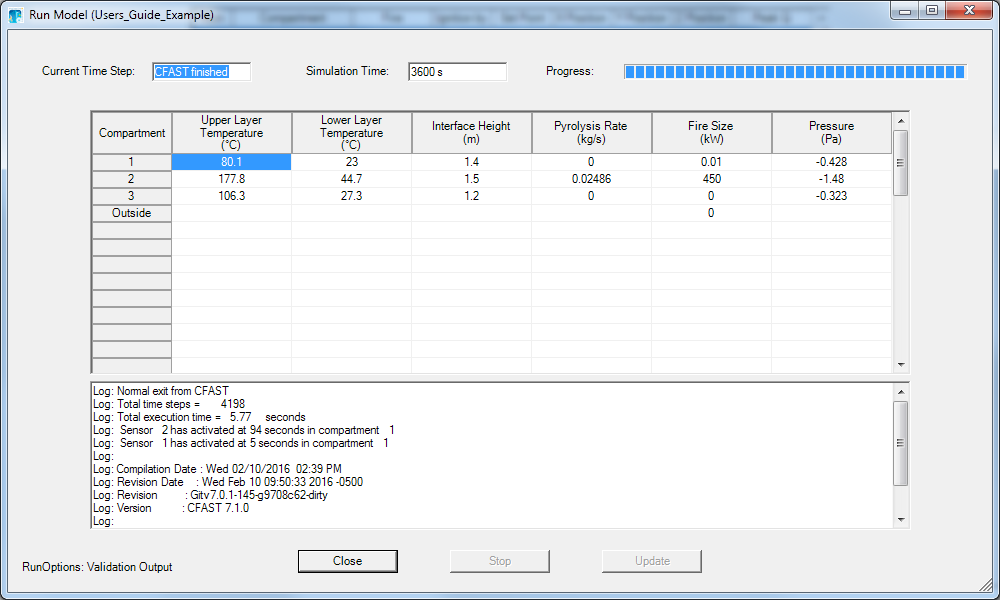
\includegraphics[width=6.5in]{FIGURES/Standard_Output}
\caption[The Standard CFAST Output Screen]{The Standard CFAST Output Screen.}
\label{Run_Model}
\end{figure}


\section{Basic Features}

The input parameters are organized via tabs near the top of the CEdit window, as shown in Fig.~\ref{primary_screen}. The tabs are:
\begin{description}
\item[Simulation Environment] includes simulation time, specification of model outputs, and ambient conditions. Also included on the page is a constantly updated list of errors, warnings, and messages about the input file specification or model simulation.
\item[Thermal Properties] defines the thermal conductivity, specific heat, density, thickness and emissivity values for all materials and fuel sources used in a simulation.
\item[Compartments] defines the size, construction characteristics, and position of the compartments in a simulation.
\item[Wall Vents] define doors and windows.
\item[Ceiling/Floor Vents] define holes in the ceiling/floor.
\item[Mechanical Ventilation] defines forced air ventilation.
\item[Fires] include user specification of the initial fire source and any additional burning objects in one or more of the compartments of the simulation.
\item[Targets] provide the ability to calculate the temperature and net heat flux to objects placed and oriented arbitrarily in the structure.
\item[Detection / Suppression] defines any heat or smoke alarms and sprinklers in the compartments of the simulation.
\item[Surface Connections] allows for more detailed description of the connections between compartments in the simulation to better simulate the transfer of heat from compartment to compartment in the simulation.
\item[Visualizations] allows specification of one or more 2-D and 3-D visualizations to be added to the simulation for viewing with Smokeview. Note that these can require significant additional computational time than a basic CFAST simulation without visualizations.
\end{description}


\section{The View Menu}

The View menu allows you to view or print the input data file, output file (if the simulation has been run and a text output file generated) and the log file of the simulation. If one of the items does not exist on the user's hard disk, the selection is grayed out.
\begin{description}
\item[Select Engineering Units] allows you to select the units for input and output. By default, most outputs are in S.I. units, with temperature in Celsius.
\end{description}


\section{The Help Menu}

The Help menu accesses this user's guide, the CFAST web site, or an about dialog box that displays the user license and version of the program.




